\chapter{Brukertest}
I dette kapittelet skal teorien bak brukervennlighetstester kort presenteres og valget av brukervennlighetstest begrunnes. Deretter skal forberedelsene og gjennomføringen av brukertestene beskrives i detalj. 

\section{Brukervennlighetstester}
Det finnes ingen offisiell definisjon på hva som kjennetegner en brukervennlighetstest. Ekspert på brukeropplevelse (\acrshort{ux}) Steve Krug definerer brukervennlighetstester som \cite[~s.13]{krugRocketSurgeryMade2010}: 
\begin{displayquote}
\textit{Å observere folk som prøver å bruke det du designer/utvikler/bygger (eller noe som du allerede har designet/utviklet/bygget) med intensjonen om å gjøre det enklere for folk å bruke eller bevise at det er enkelt i bruk}.
\end{displayquote}
Det er vanlig å kategorisere brukervennlighetstester i to ulike kategorier: kvalitative og kvantitative brukertester. 
\newline
\newline
Kvalitative brukertester går ut på å innhente funn fra observasjoner som kan identifisere designfunksjoner som er enkle eller vanskelige å bruke \cite{budiuQuantitativeVsQualitative2017}. Det betyr med andre ord at målet med slike brukervennlighetstester er å få innsikt som gjør at produktet som utvikles kan forbedres \cite[~s.14]{krugRocketSurgeryMade2010}. Ettersom målet ikke er å samle inn sammenlignbar data for å kunne bevise noe, er kvalitative brukertester gjerne mer uformelle i strukturen og protokollene kan gjerne endres på under gjennomføringen hvis det ses på som nødvendig \cite[~s.14]{krugRocketSurgeryMade2010}. Slike tester gjennomføres ofte med få brukertestdeltakere der de får oppgaver som skal løses mens de forteller hva de tenker når de samhandler med applikasjonen i en såkalt tenk-høyt protokoll, slik at observatørene kan notere hva deltakerene tenker om applikasjonen \cite{HvaErThink}. 
\newline
\newline
Kvantitative brukertester går ut på å innhente målbar data for å vurdere om oppgavene var enkle eller vanskelige å utføre \cite{budiuQuantitativeVsQualitative2017}. Det vil si at målet med kvantitative brukertester er å bevise noe ved å samle inn data som kan måles, slik som suksessrate, tid eller antall feil for å kunne trekke en konklusjon \cite[~s.13]{krugRocketSurgeryMade2010} \cite{budiuQuantitativeVsQualitative2017}. Derfor har slike brukertester en mye mer gjennomtenkt og strukturert testprotokoll som skal følges konsekvent for alle deltakere. Dette gir også et større behov for mange testdeltakere for å kunne trekke statistiske konklusjoner \cite[~s.13]{krugRocketSurgeryMade2010} .
\newline
\newline
I fordypningsprosjektet ble brukertester utført for å konkludere hvilket brukertest var best egnet for registrering av sau i blinde ved å samle data på hvor lang tid deltakerne brukte på å registrere, feilrate og tilbakemeldinger fra deltakerene hentet fra en spørreundersøkelse med spørsmål fra \acrfull{sus}. Disse testene var dermed i hovedsak kvantitative brukertester med elementer fra kvalitative brukertester ettersom spørreundersøkelsen gitt til deltakerne ble utformet for å hente kvalitative tilbakemeldinger for å forbedre funksjonaliteten i applikasjonen til den videre utviklingen under masteroppgaven. Under brukertestene for masteroppgaven skal deltakerne teste hele systemet for å finne ut hva som kan forbedres i applikasjonen. Disse testene er derfor kvalitative brukervennlighetstester. 

\section{Gjennomføring av brukertest}
Selv om kvalitative brukertester er mindre strukturerte og mer uformelle enn kvantitative brukertester, ble det utformet en plan for hvordan brukertestene skulle gjennomføres. Dette var for å forsikre at alle funksjonene som det var ønskelig å få tilbakemelding på skulle utføres av deltakerne og at samme rute ble fulgt ettersom applikasjonens GPS-funksjonalitet også skulle utprøves i testene. Det ble i tillegg bestemt at det ikke var nødvendig å teste grensesnittet for registrering i blinde ettersom det allerede var gjennomført og vurdert i fordypningsprosjektet.

\subsection{Valg av testdeltakere}
Med kvalitative brukertester er det ikke behov for mange testdeltakere ettersom det fleste store feil vil bli oppdaget tidlig og videre testing på flere deltakere vil ikke gi mer innsikt \cite[~s.43]{krugRocketSurgeryMade2010} \cite{budiuQuantitativeVsQualitative2017, renwickHowManyParticipants2019}. Det vanligste antallet testedeltakere for kvalitative tester er 5 \cite[~s.43]{krugRocketSurgeryMade2010} \cite{budiuQuantitativeVsQualitative2017, renwickHowManyParticipants2019}, og dette ble brukt som utgangspunkt for brukertestene for masteroppgaven. Opprinnelig var det ønsket å utføre brukertestene på minst én saubonde for å undersøke om applikasjonen innfridde deres behov under oppsynsturer, men på grunn av den pågående koronaviruspandemien ble dette vanskelig (les mer i underkapittelet \enquote{\nameref{korona}}). Dermed måtte brukertesten testes på utviklerenes eksisterende nærkontakter. Enkelte av disse hadde vært med i gjennomføringen av brukertestene for fordypningsoppgaven som gikk ut på å teste grensesnittet for registrering. I disse brukertestene fikk testdeltakerne en demonstrasjon og innføring i hvordan registreringen fungerte i applikasjonen, og disse deltakerne var dermed godt kjent med dette grensesnittet. Dette ble sett på som en mulighet til å undersøke om det var en forskjell mellom brukerne som tidligere var kjent med grensesnittet for registrering og brukere som ikke fikk demonstrasjon i det hele tatt. Det ble derfor valgt ut 2 deltakere som ikke hadde kjennskap til applikasjonen og 3 deltakere som hadde vært med på tidligere brukertester og var kjent med deler av brukergrensesnittet. Ellers ble ingenting annet lagret om testdeltakernes demografi, som kjønn eller alder av hensyn til personvern.

\subsection{Før testen}
En av utviklerene vil få rollen som forsøksleder og den andre som observatør, og dette avgjøres før testen. Forsøkslederens ansvar er å informere deltakere om hvordan testen skal foregå og følge planen som er utarbeidet for gjennomføringen av brukertesten slik at det blir utfort på riktig måte. Observatøren skal under hele testens forløp observere deltakerne og notere deres kommentarer på en strukturert og oversiktlig måte. For å forsikre at ble startet på like premisser, ble det utformet en sjekkliste som skulle utføres på før selve brukertesten: 
\begin{enumerate}
    \item Fjerne tidligere oppsynsturer som er blitt gjennomført på testbrukeren. 
    \item Fjerne tidligere kartutsnitt.
    \item Skru av skjermsparer
    \item Desinfisere mobiltelefonen (mer om smittevernstiltak er utdypet i kapt. \ref{korona}).
\end{enumerate}
\noindent
For å være sikker på at alle testdeltakerne fikk lik informasjon om hvordan testen skal foregå, ble det også utformet et skriv som forsøksleder leser opp fra før testen gjennomføres: 
\begin{enumerate}
    \item Forsøksleder introduserer seg selv og observatøren.
    \item Forsøksleder forklarer hensikten med brukerstesten: 
    \newline
    \textit{"Jeg vil at du skal se for deg at du er en sauebonde, og du skal sjekke hvordan det står til med saueflokken din som er på utmarksbeite for sommeren. Det er viktig at du raskt oppdager om det er skadet, død eller rovdyr på beitet slik at du kan griper inn med tiltak.
    På oppsynsturer skal du sjekke hvor mange sauer det er totalt, hvor mange sauer det er av hver farge, antall søyer og lam og antall sauer som har slips (som er en krage rundt halsen med farge som viser hvor mange lam en søye skal ha) og sauenes øremerker. Problemet er at disse sauene ofte går langt og beveger seg hele tiden, så det er en utfordring å få øye på dem. Derfor foregår registrering av sau som oftest mens man observerer sauene gjennom kikkert. I tillegg vil observasjoner av skadet, død sau eller rovdyr bli registrert dersom det oppdages på turen. I denne brukertesten skal du teste en applikasjon som skal bistå som verktøy for å registrere oppsynsturer for sau."}
    \newline
    \newline
    \textbf{Husk at det er systemet vi evaluerer og tester, ikke deg. Vi skal ikke teste hvor flink du er til å bruke appen, men hvor bra appen fungerer for deg.}
    \item Forsøksleder forklarer hvordan brukertesten gjennomføres:
    \newline
    \textit{"Vi har laget en rute for en oppsynstur der vi vil gi deg oppgaver som du skal løse med appen underveis. Det vil være 8 oppgaver til sammen.  Du kan bryte brukertesten når som helst. Si gjerne hva du tenker mens du løser oppgavene. Hvis du sliter og sitter fast med en oppgave, kan du spørre om hjelp fra forsøksleder, ellers vil ikke forsøksleder eller observatør kommentere underveis."}
    \item Deltakeren får mulighet til å spørre spørsmål og om noe er uklart.
\end{enumerate}

\subsection{Selve brukertesten} \label{brukertest}
Brukertestene ble gjennomført ved at forsøksleder, testdeltakeren og observatøren gikk en planlagt rute ved campus Gløshaugen i Trondheim, se figur  under. Forsøksleder ga testdeltakeren oppgaver underveis, og det var tilsammen 8 oppgaver med tilhørende deloppgaver som skulle utføres under turen:

\begin{figure}[H]
\centering
\captionsetup{width=.8\linewidth}
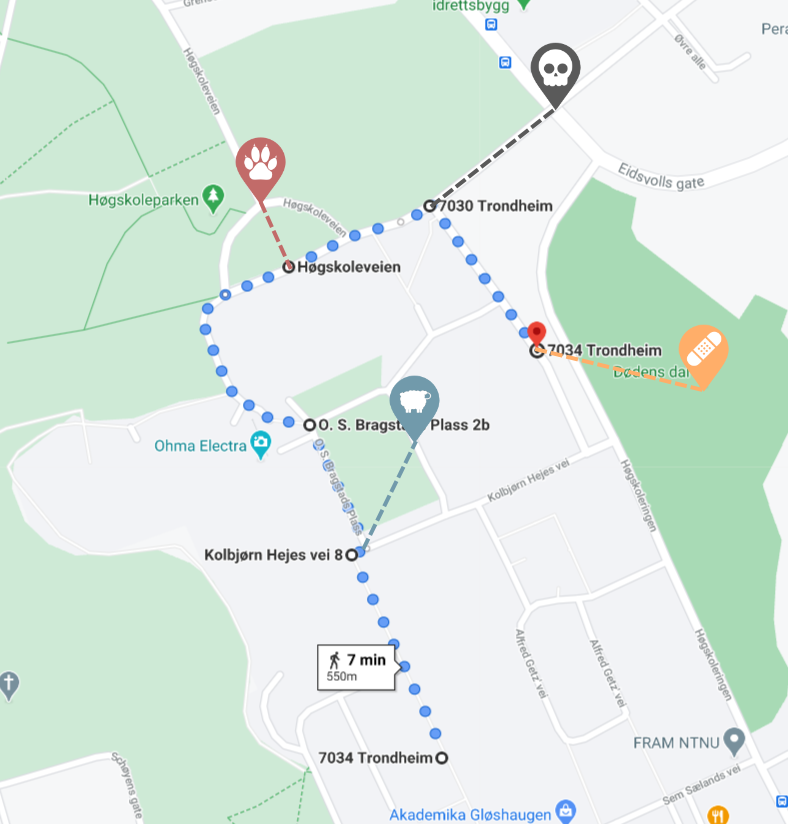
\includegraphics[scale=0.5]{Figurer/Bilder/brukertest_rute_med_pins.png}
\caption{Rute for brukertestene på Gløshaugen campus}
\label{fig:brukertest_rute}
\end{figure}
 
\renewcommand{\labelenumii}{\theenumii}
\renewcommand{\theenumii}{\theenumi.\arabic{enumii}.}
\begin{enumerate}[font=\bfseries]
    \item \textbf{Last ned kartutsnitt}
    \begin{enumerate}
        \item Endre navnet på det nedlastede kartutsnittet. 
    \end{enumerate}
    \item \textbf{Ny oppsynstur}
    \begin{enumerate}
        \item Legg til alle deltakere som er med på turen (testdeltaker, forsøksleder og observatør).
        \item Skriv inn beskrivelse om ønskelig.
    \end{enumerate}
    \item \textbf{Registrere sauer}
    \begin{itemize}
        \item Gå til Kolbjørn Hejes vei 8. Registrer sauer ved toget på andre siden av plenen.
        \begin{enumerate}
            \item 5 sauer totalt.
            \item 3 hvite, 1 svart og 1 brun.
            \item 2 søyer og 3 lam.
            \item 1 grønt og 1 gul slips.
            \item Registrer nytt øremerke med navn og farge og velg dette øremerket.
            \item Fullfør registreringen.
        \end{enumerate}
    \end{itemize}
    \item \textbf{Registrer rovdyr}
    \begin{itemize}
        \item Gå til 7034 Trondheim. Registrer rovdyr på fotballbanen.
        \begin{enumerate}
            \item Registrer observasjon av gaupe.
            \item Skriv kommentar om ønskelig.
        \end{enumerate}   
    \end{itemize}
    \item \textbf{Registrer død sau}
    \begin{itemize}
        \item Gå til trappene ved hovedbygningen. Registrer død sau ved krysset nedenfor. 
        \begin{enumerate}
            \item 1 dødt dyr.
            \item Skriv kommentar om ønskelig.
            \item Ta et bilde.
            \item Fjern bildet.
            \item Fullfør registrering.
        \end{enumerate}
    \end{itemize}
    \item \textbf{Registrer skadet sau}
    \begin{itemize}
        \item Gå til 7030 Trondheim. Registrer skadede sauer på broa rett fram.  
        \begin{enumerate}
            \item Registrer 2 skadede sau.
            \item Skriv kommentar om ønskelig.
        \end{enumerate}
    \end{itemize}
    \item \textbf{Fullfør oppsynstur}
    \begin{enumerate}
        \item Sjekk om registreringene stemmer.
        \item Oppdater beskrivelse om ønskelig.
        \item Trykk "Fullfør". 
    \end{enumerate}
\end{enumerate}

\subsection{Etter testen}
Etter testen ble testdeltakerne spurt om de hadde noen generelle tilbakemeldinger og deres helhetlige inntrykk av applikasjonen. 

\subsubsection{Gjennomføring av brukertest under Covid-19} \label{korona}
Gjennomføringen av brukertestene har vært sterkt preget av den pågående Covid-19 pandemien for både fordypningsprosjektet og masteroppgaven. Selv om det var svært lite smitte i Trondheim da brukertestene skulle gjennomføres, ble det innført strenge nasjonale smittevernstiltak 23.03.21, dagen før det var planlagt å utføre brukertestene. Økt avstand og færre nære kontakter er to sentrale smittereduserende tiltak i håndteringen av koronapandemien ifølge \acrfull{fhi} \cite{AvstandOgFaerre2020}. Derfor ble det tatt noen forholdssregler og iverksatt smittevernstiltak under selve brukertestene slik at brukertestene ble gjennomført på en trygg måte og tilfredstilte \acrshort{fhi} sine råd og anbefalinger. Det ble bestemt at alle testdeltakerne skulle være venner som allerede ble betegnet som utviklerens nærkontakter slik at ingen utenforstående eller utviklerne selv måtte bli utsatt for særskilt risiko. Dette medførte at alle testdeltakerne var medstudenter i 20-årene. For å få best mulig data ville det vært mer optimalt med en jevnere demografisk spredning av deltakerne og testing av faktiske sauebønder, men det ble uaktuelt i en slik smittesituasjon. I tilegg ble det også utført praktiske smittevernstiltak for å sørge for at brukertestene ble tryggest mulig. Mobiltelefonen som testdeltakerne benyttet seg av i brukertestene ble desinfisert før og etter testen og utviklerne sørget for å holde minst 2 meter avstand slik de daværende smittereglene anbefalte. 

\section{Konklusjon}
Det ble utført brukervennlighetstester på Sauron for å få tilbakemeldinger på hvor godt egnet applikasjonen er til å bistå i registrering av sau på oppsynstur. Testene som ble gjennomført var såkalte kvalitative tester med fokus på å avdekke problemområder i designen og funksjonaliteten til applikasjonen. Det ble utformet en plan og rute for gjennomføringen av brukertestene som ble fulgt. Tilsammen 5? personer ble testet. På grunn av den pågående Covid-19 ble det satt smittevernstiltak og begrensninger for brukertestene, særlig for demografien til testdeltakerne. 